\section{Odd Elastodynamics III}

\subsection{Review}
We continue our discussion of odd elastodynamics. Last time, we considered the limit where $G, B, A \ll K^0$ and where we had overdamped dynamics. We then showed that we have oscillations with frequency:
\begin{equation}
    \omega = \frac{K^0}{\Gamma}q^2
\end{equation}
Remarkably, we get standing waves, where stress and strain are 90 degrees out of phase (Figure below taken from \url{https://www.nature.com/articles/s41567-020-0795-y}).

\begin{center}
    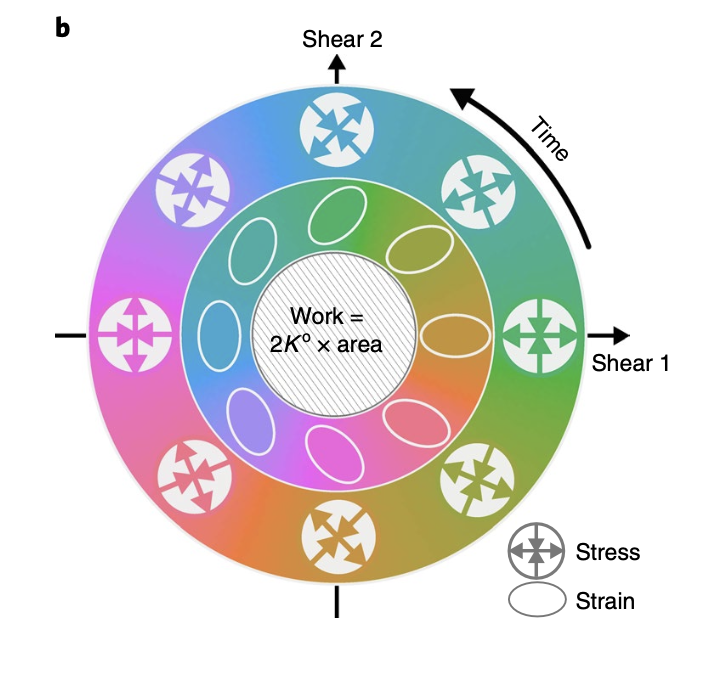
\includegraphics[scale=0.5]{Lectures/Images/lec6-oddelasticwave.png}
\end{center}

In strain space, we trace out an area, corresponding to work:
\begin{equation}
    W = 2K^0 \text{Area}
\end{equation}
with wave speed:
\begin{equation}
    c = \frac{2K^0q}{\Gamma}.
\end{equation}

Decomposing the displacements into parallel and perpendicular components:
\begin{equation}
    u_\parallel \equiv \hat{q}_i\tilde{u}_i, \quad u_\perp \equiv \e_{ij}\hat{q}_j \tilde{u}_i
\end{equation}
we obtain the relation:
\begin{equation}
    -i\omega\Gamma\m{u_\parallel \\ u_\perp} = -q^2\m{B + G & K^0 \\ -K^0 - A & G}\m{u_\parallel \\ u_\perp}
\end{equation}
which inform us about the normal modes of the elastic spectrum. We will momentarily see how the dynamical matrix for an odd solid differs from a regular one - namely the matrix is not Hermitian. We want to use the above matrix equation to solve for the eigenfrequencies and eigenvectors. Taking the determinant and setting it to zero, we find:
\begin{equation}\label{eq:oddnormalfreqs}
    \omega = -i\left[\underbrace{\frac{B}{2} + G}_{\text{decay}} \pm \sqrt{\left(\frac{B}{2}\right)^2 - K^0A - (K^0)^2}\right]\frac{q^2}{\Gamma}
\end{equation}

The decay term comes from the fact that the odd elasticity tries to deform the object, but this costs energy in terms of the bulk/shear modulus (because it strains the material). The more we pay that energy cost (i.e. larger $B, G$) the more the wave gets attenuated. Fortunately, we look at the $B, G \ll K^0$ limit; this is somewhat equivalent to studying fluid density waves in the low-viscosity limit. Microscopically this is quite odd (though there are some physical systems, e.g. Abrikosov lattices in superconductors), because this corresponds to the $\kappa \to 0$ limit of the microscopic force law $F = -(\kappa^0\hat{\gv{\phi}} + \kappa\rhat)\delta r$. 

We can study the onset of waves; this occurs when we have $e^{i\text{Re}(\omega)t}$, but this only occurs when the argument of the square root is negative. The condition we found was:
\begin{equation}
    1 - \tilde{K}^0\tilde{A} - (\tilde{K}^0)^2 < 0
\end{equation}
where $\tilde{K}^0 = \frac{2K^0}{B}, \tilde{A} = \frac{2\tilde{A}}{B}$. The locus/phase transition was given by the hyperbola:
\begin{equation}
    \tilde{A} = \frac{1}{\tilde{K}^0} - \tilde{K}^0
\end{equation}

\subsection{Instability, Phase Diagram}
Notice the heuristic argument we made based on energy balance relied on the argument that the energy produced in one cycle could overcome the dissipation lost. In particular, we set the energy gained to be equal to that lost. If the energy gained was less, then the wave would die out. If the energy gained was more, then instead we would have an instability/the wave amplitude would continue to grow.

Let's look at the region of this instability more carefully. This occurs when the spectrum acquires a positive imaginary branch. In particular, we look for a situation where $e^{\Im(\omega)t}$ with $\Im(\omega) > 0$, then we have exponential amplification in time. We require:
\begin{equation}
    \frac{B}{2} + G - \sqrt{\left(\frac{B}{T}\right)^2 - K^0A - (K^0)^2} < 0
\end{equation}
then the crossover happens when:
\begin{equation}
    \left(1 + \tilde{G}\right)^2 = 1 - \tilde{K}^0\tilde{A} - (\tilde{K}^0)^2
\end{equation}
i.e.:
\begin{equation}
    \tilde{A} = -\frac{2\tilde{G} +\tilde{G}^2 + (\tilde{K}^0)^2}{\tilde{K}^0}
\end{equation}
Note that we know that we have instability after this point - we don't know what happens after this (whether we get nonlinear excitations, or whether the lattice begins to melt/crumble etc...)

With this region discussed, we can now understand the entire phase diagram (figure taken from \url{https://www.nature.com/articles/s41567-020-0795-y})

\begin{center}
    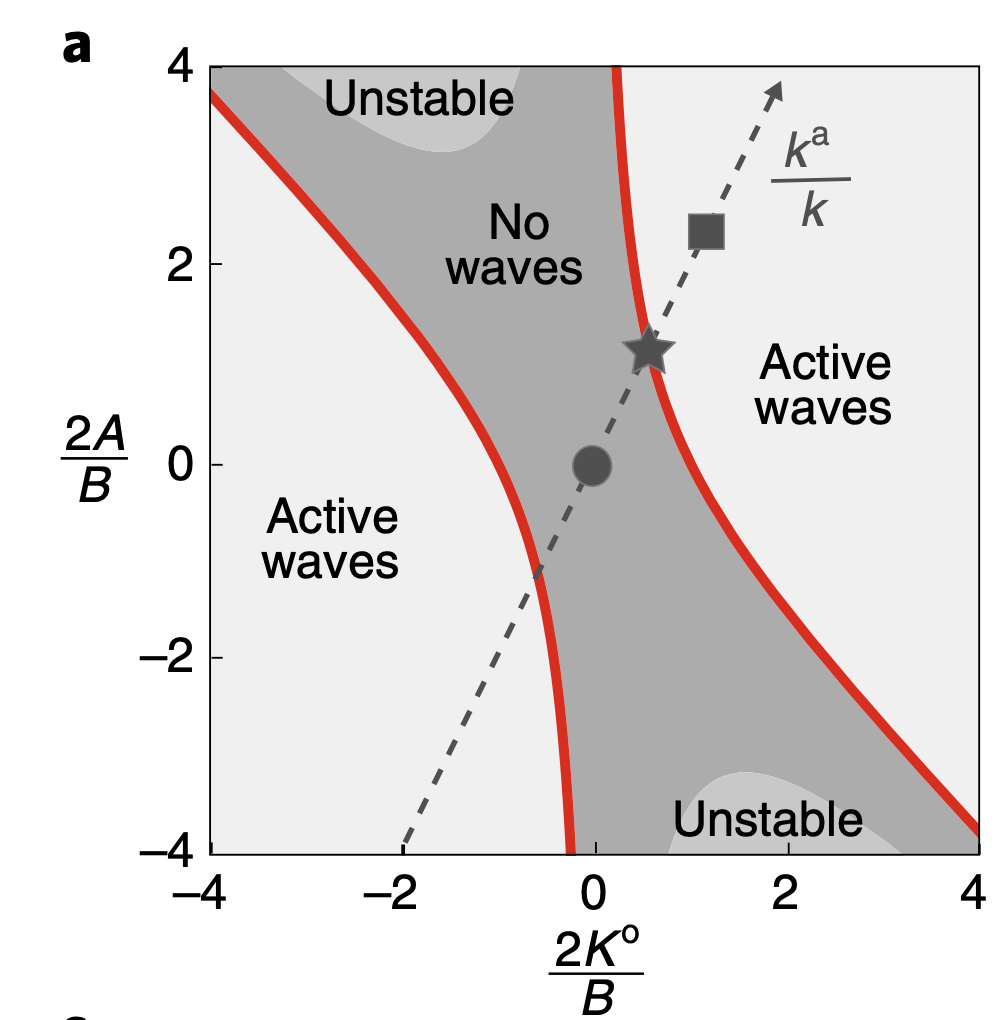
\includegraphics[scale=0.5]{Lectures/Images/lec6-oddelasticphasediagram.png}
\end{center}

A comment; if we had assumed a microscopic force model of $F = -(\kappa^0\hat{\gv{\phi}} + \kappa \rhat)\delta r$, we could course grain to find the dependencies of $A, K^0, B$ on the microscopic parameters, and then the knowledge of the microscopic parameter ratio $\frac{\kappa^0}{\kappa}$ would be able to tell us about where in the phase diagram we were located.

Another comment about instability: even if we have a linear microscopic constitutive equation, we could potentially get macroscopic non-linearities coming out of rotations (only 2-d and up - coming from the last term):
\begin{equation}
    u_{ij} = \p_i u_j + \p_j u_i + \p_k u_i \p_k u_j.
\end{equation}



\subsection{Exceptional Points}
Now, let's talk about what happens on the dashed line of the phase diagram when we cross from the active to the no wave region (star point). We have the $\omega$ from Eq. \eqref{eq:oddnormalfreqs}, and can also compute the eigenvectors. Before, this, a comment about the dynamical matrix - It is not Hermitian if $A, K^0 \neq 0$. This means that the convenient properties - real eigenvalues, orthogonal eigenvectors - are lost. In QM this is necessary for real measurement outcomes and conservation of probability. But for open quantum systems, we require non-Hermitian matrices. 

Let's compute the eigenvectors and see that they are non-orthogonal:
\begin{equation}
    u_i = \frac{(1 \pm \sqrt{1 - \tilde{K}^0\tilde{A} - (\tilde{K}^0)^2})\hat{q}_i - (\tilde{A} + \tilde{K}^0)\e_{ij}\hat{q}_j}{\sqrt{2(1\pm\sqrt{1 - \tilde{K}^0\tilde{A} - (\tilde{K}^0)^2}) + \tilde{K}^0\tilde{A} + (\tilde{K}^0)^2}}
\end{equation}
Unwieldy, but you might be able to convince yourself that we only get orthogonality if $\tilde{K}^0 = A = 0$.

With this obtained we can discuss what happens at the onset of odd waves. There is a point called the \emph{exceptional point}\footnote{In this age of exceptionalism, Vincenzo must apologize and say that this is not that exceptional.}. It is a statement about the fact that a singularity occurs.

\begin{enumerate}[(a)]
    \item We can see from Eq. \eqref{eq:oddnormalfreqs} that at the exceptional point when $\tilde{A} = \frac{1}{\tilde{K}^0} - \tilde{K}^0$ that the square root term is zero and that the spectrum acquires a degeneracy, where the eigenvalues become the same:
    \begin{equation}
        \omega = -i\left[\frac{B}{2} + G \pm 0\right]
    \end{equation}
    \item What happens to the $u_+, u_-$ eigenvectors at this point? They become collinear!
\end{enumerate}

We will encounter these exceptional points again when we study non-reciprocal phase transitions.

\subsection{Poisson Ratio and Odd Ratio}
Imagine we could measure the spectrum of the odd waves; we would be able to measure $\tilde{K}^0, A, \frac{B}{2}, G$ etc. This would be a dynamical measurement. You might also ask - why could we not do a static measurement? Indeed we could just compress/apply forces to the solid in different ways, and just see how it deforms.

We can consider the Poisson ratio:
\begin{equation}
    \nu = -\frac{u_{xx}}{u_{yy}}
\end{equation}
in normal materials, $\nu > 0$ and so if we compress one way, it expands in the other direction. In auxetic materials (e.g. metamaterials like rotating triangular auxetic perforated plates), we have $\nu < 0$ so if we compress it compresses in the other direction too! There is also the case of $\nu \approx 0$, e.g. cork where we compress in one direction and the other direction basically does not change. 

What about odd materials? we compress in one direction and then there is a response to an angle. This violates parity - and hence requires parity violating moduli. Note that in this case it is useful to define the odd ratio:
\begin{equation}
    \nu^0 = \frac{K^0B}{(K^0)^2 + G^2 + BG}
\end{equation}
which characterizes the angle at which the material deforms when compressed.

Next time, we look at the case where linear momentum conservation is violated. Then we turn to fluids without viscosity, in particular turbulence in non-viscous fluids.